\documentclass[letterpaper,10pt]{article}
\usepackage[margin=0.75in]{geometry}
\usepackage[T1]{fontenc}
\usepackage{lmodern}
\usepackage{amsmath}
\usepackage{booktabs}
\usepackage{longtable}
\usepackage{array}
\usepackage{float}
\usepackage{cite}
\usepackage{graphicx}
\usepackage{pdfpages}
\usepackage{fvextra}

\usepackage{ragged2e}
\usepackage{pdflscape}
\usepackage{xurl}
\usepackage[hidelinks]{hyperref}

\newcolumntype{L}[1]{>{\RaggedRight\arraybackslash}p{#1}}

\setlength{\parindent}{0pt}
\setlength{\parskip}{0.45em}
\renewcommand{\arraystretch}{1.08}

\title{Supplementary Clinical-Evidence Corroboration}
\author{}
\date{}

\begin{document}
\maketitle
\small

\section{Complete Original-Cohort Estimator Matrix}

Table~\ref{tab:supp-original-cate} reports every prespecified original-cohort
dataset--exposure comparison for CausalForestDML, LinearDML, and CausalPFN.
Values are retained irrespective of magnitude, direction, or cross-estimator
agreement. The table reports mean model-estimated CATE summaries over each
analyzed sample; these are not ground-truth causal effects.

\begin{longtable}{@{}p{0.84in}p{1.42in}rrrp{0.68in}@{}}
\caption{Complete original-cohort estimator summaries (CF-DML denotes
CausalForestDML). Values are mean model-estimated CATE summaries over the
analyzed samples; display precision is six decimal places.}
\label{tab:supp-original-cate}\\
\toprule
Dataset & Exposure & CF-DML & LinearDML & CausalPFN & Sign agreement\\
\midrule
\endfirsthead
\toprule
Dataset & Exposure & CF-DML & LinearDML & CausalPFN & Sign agreement\\
\midrule
\endhead
MIMIC-III & Cardiac strain
& +0.220356 & +0.187634 & +0.259327 & all three\\
MIMIC-III & Inflammation/sepsis
& +0.161179 & +0.161334 & +0.148544 & all three\\
MIMIC-III & Hepatic/coag.\ dysfunction
& +0.097598 & +0.083017 & +0.096846 & all three\\
MIMIC-III & Renal dysfunction
& +0.091290 & +0.088595 & +0.086972 & all three\\
MIMIC-III & Global severity
& +0.062101 & +0.080153 & +0.073050 & all three\\
MIMIC-III & Respiratory failure
& +0.036133 & +0.039098 & +0.049766 & all three\\
MIMIC-III & Neurologic dysfunction
& +0.034253 & +0.031550 & +0.034993 & all three\\
MIMIC-III & Shock
& +0.020994 & +0.021246 & +0.031645 & all three\\
MIMIC-III & Metabolic derangement
& +0.019743 & +0.017989 & +0.031323 & all three\\
\addlinespace
PhysioNet 2012 & Renal dysfunction
& +0.120027 & +0.090622 & +0.110669 & all three\\
PhysioNet 2012 & Cardiac injury/strain
& +0.111831 & +0.122033 & +0.119413 & all three\\
PhysioNet 2012 & Global severity
& +0.107988 & +0.106740 & +0.105039 & all three\\
PhysioNet 2012 & Hepatic dysfunction
& +0.090527 & +0.060184 & +0.106843 & all three\\
PhysioNet 2012 & Neurologic dysfunction
& +0.081636 & +0.075728 & +0.077049 & all three\\
PhysioNet 2012 & Metabolic derangement
& +0.077704 & +0.079738 & +0.090734 & all three\\
PhysioNet 2012 & Inflammation/sepsis burden
& +0.071800 & +0.070872 & +0.067480 & all three\\
PhysioNet 2012 & Respiratory failure
& +0.064750 & +0.062660 & +0.062984 & all three\\
PhysioNet 2012 & Coag./heme dysfunction
& +0.010794 & +0.004136 & +0.025428 & all three\\
PhysioNet 2012 & Shock
& -0.013849 & -0.026944 & +0.004122 & disagreement\\
\bottomrule
\end{longtable}

\begin{landscape}

\section{Clinical Evidence Used to Construct the Proxy Exposures}
\label{sec:supp-proxy-definitions}

Table~\ref{tab:supp-proxy-definitions} documents the 19 admitted proxy
exposures used by CliniCause: nine in MIMIC-III and ten in PhysioNet 2012.
Only sources explicitly recoverable from the preserved ChatGPT responses are
called \emph{ChatGPT-supplied}. Later literature checks are identified
separately and must not be interpreted as original prompt provenance. The rules
below are analytical proxy definitions rather than chart-adjudicated diagnoses;
a cited source may support the broad clinical construct or an individual clause
without validating the complete local Boolean composite.

\scriptsize
\setlength{\tabcolsep}{2.2pt}
\renewcommand{\arraystretch}{1.08}

\begin{longtable}{@{}L{0.88in}L{1.72in}L{2.32in}L{1.05in}L{2.82in}@{}}
\caption{Proxy-definition evidence for all admitted CliniCause exposures. Each
row reports the implemented source columns, exact cutoff and aggregation rule,
clinical interpretation, and the preserved ChatGPT source evidence with a
bounded support paraphrase and DOI or stable URL.}
\label{tab:supp-proxy-definitions}\\
\toprule
Dataset/proxy &
Source columns &
Exact cutoff, combination, and aggregation rule &
Clinical interpretation &
ChatGPT-supplied support, DOI/URL, and evidence qualification \\
\midrule
\endfirsthead

\toprule
Dataset/proxy &
Source columns &
Exact cutoff, combination, and aggregation rule &
Clinical interpretation &
ChatGPT-supplied support, DOI/URL, and evidence qualification \\
\midrule
\endhead

MIMIC-III M01\newline Inflammation/\newline sepsis &
Temperature min/max; WBC min/max; lactate max; culture ordered/positive;
suspected infection; antibiotic started/any. &
Five indicators: temperature $\geq38.3$ or $<36$; WBC $>12$ or $<4$;
lactate $>2$; culture or suspected-infection evidence; antibiotic or
suspected-infection evidence. Positive when score $\geq2$ and a culture,
antibiotic, temperature, or WBC anchor is present. Whole available ICU record
summaries; missing clauses do not fire. &
Inflammation or suspected-infection/sepsis burden; not confirmed sepsis. &
Original ChatGPT source: Sepsis-3,
\href{https://doi.org/10.1001/jama.2016.0287}
{doi:10.1001/jama.2016.0287}. It supports infection-related dysregulated host
response and organ dysfunction, but not this five-clause score or its exact
threshold. \\
\addlinespace

MIMIC-III M02\newline Global severity &
MAP/SBP; vasopressor; SpO$_2$; P/F ratio; ventilation; GCS/RASS;
creatinine/urine; lactate/pH/bicarbonate; temperature/WBC;
bilirubin/platelets/INR. &
Seven Boolean domains: circulatory, respiratory, neurologic, renal, metabolic,
inflammatory, and hepatic/coagulation. Positive when at least three domains are
abnormal. Whole-record extrema/first values and any-flags; urine uses first
24 h and minimum rolling 6 h summaries; missing clauses do not fire. &
Multi-domain acute physiological severity. &
Original ChatGPT source: MSD SOFA table,
\url{https://www.msdmanuals.com/professional/multimedia/table/sequential-organ-failure-assessment-sofa-score}.
Later verification: original SOFA paper,
\href{https://doi.org/10.1007/BF01709751}{doi:10.1007/BF01709751}.
These support six organ domains and daily worst values, not the local
seven-domain Boolean score or cutoff of three. \\
\addlinespace

MIMIC-III M03\newline Shock &
MAP/SBP; sustained MAP $<70$ flag; vasopressor; lactate; 24 h and rolling
6 h urine; pH; base excess. &
Five indicators: MAP $<65$, SBP $\leq90$, or sustained MAP $<70$;
vasopressor; lactate $>2$; urine $<0.5$ mL/kg/h over 6 h or
$<500$ mL/24 h; pH $<7.30$ or base excess $\leq-5$. Positive when score
$\geq2$, or vasopressor plus hypoperfusion, acidosis, or hypotension.
Whole-record aggregation; missing clauses do not fire. &
Circulatory shock or clinically meaningful hemodynamic instability. &
Original ChatGPT sources: Sepsis-3,
\href{https://doi.org/10.1001/jama.2016.0287}
{doi:10.1001/jama.2016.0287}, and the MSD SOFA table,
\url{https://www.msdmanuals.com/professional/multimedia/table/sequential-organ-failure-assessment-sofa-score}.
They support vasopressor-dependent hypotension, lactate $>2$, and
cardiovascular-dysfunction concepts, not the project's broader any-two
composite. \\
\addlinespace

MIMIC-III M04\newline Respiratory\newline failure &
SpO$_2$; P/F ratio; FiO$_2$; invasive/non-invasive ventilation; respiratory
rate; PaCO$_2$; pH. &
Five indicators: SpO$_2<92$; P/F $\leq300$; respiratory support or
FiO$_2\geq0.5$; respiratory rate $\geq30$ or $\leq8$;
PaCO$_2\geq50$ with pH $<7.30$. Positive when score $\geq2$, or support
plus hypoxemia, low P/F, or ventilatory failure. Whole-record aggregation;
missing clauses do not fire. &
Hypoxemic or ventilatory failure and/or substantial respiratory support. &
Original ChatGPT source: MSD Berlin-definition table,
\url{https://www.msdmanuals.com/professional/multimedia/table/berlin-definition-of-ards}.
Later verification: Berlin definition,
\href{https://doi.org/10.1001/jama.2012.5669}
{doi:10.1001/jama.2012.5669}. It supports P/F severity categories under
PEEP/CPAP together with timing, imaging, and edema-origin requirements; the
project proxy is broader and is not an ARDS diagnosis. \\
\addlinespace

MIMIC-III M05\newline Renal\newline dysfunction &
Creatinine max/delta; BUN; 24 h and rolling 6 h urine; potassium;
bicarbonate; dialysis/CRRT. &
Five indicators: creatinine $\geq2$ or rise $\geq0.3$; BUN $\geq40$;
urine $<0.5$ mL/kg/h over 6 h or $<500$ mL/24 h; potassium $\geq5.5$
or bicarbonate $<18$; dialysis. Positive when score $\geq2$ or dialysis is
present. Whole-record aggregation; missing clauses do not fire. &
Acute or clinically important renal dysfunction. &
Original ChatGPT source: MSD KDIGO staging table,
\url{https://www.msdmanuals.com/professional/multimedia/table/staging-criteria-for-acute-kidney-injury-kdigo-2012}.
Later verification: KDIGO AKI guideline,
\url{https://kdigo.org/guidelines/acute-kidney-injury/}. These support a
$0.3$ mg/dL creatinine rise, baseline-relative change, and timed urine
criteria, not the BUN/electrolyte composite or its any-two rule. \\
\addlinespace

MIMIC-III M06\newline Hepatic/coag.\newline dysfunction &
Bilirubin; AST/ALT; platelets; INR; prolonged PT/PTT; albumin. &
Five indicators: bilirubin $\geq2$; AST or ALT $\geq120$; platelets
$<100$; INR $\geq1.5$ or prolonged PT/PTT; albumin $<2.5$. Positive
when score $\geq2$. Whole-record aggregation; missing clauses do not fire. &
Combined hepatic injury/reserve and coagulation dysfunction. &
Original ChatGPT source: MSD SOFA table,
\url{https://www.msdmanuals.com/professional/multimedia/table/sequential-organ-failure-assessment-sofa-score};
later verification used the original SOFA paper,
\href{https://doi.org/10.1007/BF01709751}{doi:10.1007/BF01709751}.
SOFA supports bilirubin and platelet domains separately, not this combined
five-indicator score. \\
\addlinespace

MIMIC-III M07\newline Neurologic\newline dysfunction &
GCS; abnormal GCS components; RASS; pupil/focal-neurologic abnormality;
sedation/intubation context. &
GCS $\leq8$ contributes 2; otherwise GCS $\leq13$ contributes 1.
Abnormal GCS component, RASS $\leq-3$ or $\geq2$, and pupil/focal
abnormality each contribute 1. Positive when score $\geq2$;
sedation/intubation with an isolated one-point score is forced negative.
Whole-record aggregation; missing clauses do not fire. &
Depressed consciousness or focal/behavioral neurologic dysfunction. &
Original ChatGPT source: MSD SOFA table,
\url{https://www.msdmanuals.com/professional/multimedia/table/sequential-organ-failure-assessment-sofa-score};
later verification:
\href{https://doi.org/10.1007/BF01709751}{doi:10.1007/BF01709751}.
SOFA supports GCS as the neurologic domain, not the RASS/focal-sign weighting
or sedation exclusion. \\
\addlinespace

MIMIC-III M08\newline Metabolic\newline derangement &
pH; bicarbonate; base excess; lactate; potassium; sodium; glucose. &
Six domains: pH $<7.30$ or $>7.55$; bicarbonate $<18$ or $>35$ or
base excess $\leq-5$; lactate $>2$; potassium $<3$ or $\geq5.5$;
sodium $<130$ or $>150$; glucose $<70$ or $>250$. Positive when at
least two domains are abnormal. Whole-record aggregation; missing clauses do
not fire. &
Acid-base, lactate, electrolyte, or glucose derangement. &
No proxy-specific original ChatGPT source or DOI/URL was recovered. No locally
inspected paper validates the exact six-domain score, its cutoffs, or the
any-two combination. \\
\addlinespace

MIMIC-III M09\newline Cardiac strain &
Troponin flags and maxima; CK-MB; arrhythmia; heart rate; MAP/SBP; first care
unit; cardiac-surgery context. &
Five indicators: abnormal troponin, with fallback T $\geq0.1$ or
I $\geq0.4$; abnormal CK-MB; arrhythmia or HR $>150$/$<40$;
HR $>130$ or $<40$ with hypotension; CCU/CSRU or cardiac-surgery context.
Positive when score $\geq2$ and a troponin or rhythm anchor is present.
Whole-record aggregation; missing clauses do not fire. &
Myocardial injury, rhythm instability, or severe cardiac strain. &
No proxy-specific original ChatGPT source was recovered. A later
myocardial-injury source was identified,
\href{https://doi.org/10.1161/CIR.0000000000000617}
{doi:10.1161/CIR.0000000000000617}, but it was not preserved as original
ChatGPT provenance and its full text was not available for this audit.
The assay-specific thresholds and composite remain unverified. \\

\midrule

PhysioNet P01\newline Global severity &
MAP/NIMAP/SBP; ventilation; P/F or PaO$_2$/FiO$_2$ approximation;
SaO$_2$; respiratory rate; GCS; creatinine/BUN/urine;
bilirubin/platelets; lactate/pH/HCO$_3$; troponin/HR. &
Seven domains: hemodynamic, respiratory, neurologic, renal,
hepatic/coagulation, metabolic, and cardiac. Positive when score $\geq3$, or
score $\geq2$ plus lactate $\geq4$, pH $<7.20$, ventilation,
GCS $\leq8$, or MAP $<60$. Whole first-48 h record using
min/max/mean/first/last summaries; missing clauses do not fire. &
Multi-domain first-48 h acute physiological severity. &
Original ChatGPT source: MSD SOFA table,
\url{https://www.msdmanuals.com/professional/multimedia/table/sequential-organ-failure-assessment-sofa-score};
later verification:
\href{https://doi.org/10.1007/BF01709751}{doi:10.1007/BF01709751}.
SOFA supports six organ domains and ordinal thresholds, not the local
seven-domain score or critical override. \\
\addlinespace

PhysioNet P02\newline Shock &
MAP/NIMAP/SBP; lactate; heart rate; urine summary; pH; bicarbonate. &
Six indicators: MAP or NIMAP $<70$; SBP or non-invasive SBP $\leq90$;
lactate $>2$; HR $\geq110$; urine $<500$ mL; pH $<7.30$ or
bicarbonate $<18$. Positive when score $\geq2$, or low MAP with lactate
$\geq4$. Whole first-48 h record; missing clauses do not fire. &
Circulatory shock or hemodynamic instability without vasopressor data. &
Original ChatGPT source: MSD SOFA table,
\url{https://www.msdmanuals.com/professional/multimedia/table/sequential-organ-failure-assessment-sofa-score};
later verification:
\href{https://doi.org/10.1007/BF01709751}{doi:10.1007/BF01709751}.
It supports MAP $<70$ as cardiovascular dysfunction, not the complete
any-two score or lactate override. \\
\addlinespace

PhysioNet P03\newline Respiratory\newline failure &
Ventilation; P/F or PaO$_2$/FiO$_2$ approximation; SaO$_2$/PaO$_2$;
respiratory rate; PaCO$_2$; pH. &
Five indicators: ventilation; P/F $<300$; SaO$_2<92$ or PaO$_2<60$;
respiratory rate $\geq22$ or $<8$; PaCO$_2\geq50$, or
PaCO$_2\geq45$ with pH $<7.30$. Positive when score $\geq2$, or
ventilation plus P/F $<300$. Whole first-48 h record; missing clauses do
not fire. &
Hypoxemic or ventilatory respiratory failure/support. &
Original ChatGPT source: MSD SOFA table,
\url{https://www.msdmanuals.com/professional/multimedia/table/sequential-organ-failure-assessment-sofa-score},
supporting P/F oxygenation scoring. Later verification: Berlin definition,
\href{https://doi.org/10.1001/jama.2012.5669}
{doi:10.1001/jama.2012.5669}. Neither source validates the full composite,
and the proxy is not an ARDS diagnosis. \\
\addlinespace

PhysioNet P04\newline Renal\newline dysfunction &
Creatinine first/max; BUN; urine summary; potassium; bicarbonate. &
Five indicators: creatinine $\geq2$; creatinine rise $\geq0.3$;
BUN $\geq40$; urine $<500$ mL; potassium $\geq5.5$ or bicarbonate
$<18$. Positive when score $\geq2$ or creatinine $\geq3.5$. Whole
first-48 h record; missing clauses do not fire. &
Acute or clinically important renal dysfunction. &
Original ChatGPT source: MSD SOFA table,
\url{https://www.msdmanuals.com/professional/multimedia/table/sequential-organ-failure-assessment-sofa-score}.
Later verification: KDIGO AKI guideline,
\url{https://kdigo.org/guidelines/acute-kidney-injury/}. These support
creatinine/urine domains and the $0.3$ rise, not the local full score or
sufficient condition. \\
\addlinespace

PhysioNet P05\newline Hepatic\newline dysfunction &
Bilirubin; AST/ALT; alkaline phosphatase; albumin; platelets. &
Weighted score: bilirubin $\geq2$ contributes 2; AST or ALT $\geq200$,
ALP $\geq250$, albumin $<2.5$, and platelets $<100$ each contribute 1.
Positive when score $\geq2$. Whole first-48 h record; missing clauses do
not fire. &
Cholestatic/hepatocellular injury or impaired hepatic reserve. &
Original ChatGPT source: MSD SOFA table,
\url{https://www.msdmanuals.com/professional/multimedia/table/sequential-organ-failure-assessment-sofa-score};
later verification:
\href{https://doi.org/10.1007/BF01709751}{doi:10.1007/BF01709751}.
SOFA supports bilirubin as a liver-domain marker, not the enzyme, albumin,
platelet weighting, or the local threshold combination. \\
\addlinespace

PhysioNet P06\newline Coagulation/\newline hematologic &
Platelets first/min; hematocrit min/max; WBC min/max. &
Weighted score: platelets $<100$ contributes 2; platelets $<150$,
hematocrit $<25$ or $>55$, WBC $<4$ or $>20$, and platelet drop
$\geq50$ each contribute 1. Positive when score $\geq2$. Whole first-48 h
record; missing clauses do not fire. &
Thrombocytopenia, anemia/polycythemia, or hematologic stress. &
Original ChatGPT source: MSD SOFA table,
\url{https://www.msdmanuals.com/professional/multimedia/table/sequential-organ-failure-assessment-sofa-score},
supporting platelet thresholds. Later verification used an ISTH DIC source,
\href{https://doi.org/10.1055/s-0037-1616068}
{doi:10.1055/s-0037-1616068}, which uses a different multi-test algorithm.
Neither validates the HCT/WBC additions or local weighting. \\
\addlinespace

PhysioNet P07\newline Inflammation/\newline sepsis &
Temperature; WBC; heart rate; respiratory rate; PaCO$_2$; lactate;
platelets. &
Six indicators: temperature $>38.3$ or $<36$; WBC $>12$ or $<4$;
HR $>90$; respiratory rate $>20$ or PaCO$_2<32$; lactate $>2$;
platelets $<150$. Positive when score $\geq3$, or abnormal temperature/WBC
plus lactate and score $\geq2$. Whole first-48 h record; missing clauses do
not fire. &
Systemic inflammatory or sepsis-like host response; not confirmed sepsis. &
Original ChatGPT source: Sepsis-3,
\href{https://doi.org/10.1001/jama.2016.0287}
{doi:10.1001/jama.2016.0287}. It supports infection-related organ
dysfunction and supersedes a simple inflammation-only definition; the local
record lacks an infection anchor, and the SIRS-like score is not Sepsis-3. \\
\addlinespace

PhysioNet P08\newline Neurologic\newline dysfunction &
GCS; sodium; glucose; PaCO$_2$; SaO$_2$; pH. &
GCS $\leq12$ contributes 2; GCS $<15$, sodium $<130$ or $>150$ or
glucose $<70$ or $>300$, and PaCO$_2\geq50$/SaO$_2<90$/pH $<7.25$
each contribute 1. Positive when score $\geq2$. Whole first-48 h record;
missing clauses do not fire. &
Depressed consciousness or neurologic dysfunction with metabolic/gas
contributors. &
Original ChatGPT source: MSD SOFA table,
\url{https://www.msdmanuals.com/professional/multimedia/table/sequential-organ-failure-assessment-sofa-score};
later verification:
\href{https://doi.org/10.1007/BF01709751}{doi:10.1007/BF01709751}.
SOFA supports GCS as a neurologic domain, not the added electrolyte and gas
clauses or their weighting. \\
\addlinespace

PhysioNet P09\newline Cardiac injury/\newline strain &
Troponin I/T; ICU type; heart rate; MAP/SBP; lactate. &
Weighted score: troponin I $>0.1$ or T $>0.01$ contributes 2;
ICU type 1/2, HR $\geq130$ or $<50$, MAP $<70$ or SBP $\leq90$, and
lactate $>2$ each contribute 1. Positive when score $\geq2$. Whole
first-48 h record; missing clauses do not fire. &
Myocardial injury, ischemia, or severe cardiac strain. &
No proxy-specific original ChatGPT source was recovered. A later
myocardial-injury source was identified,
\href{https://doi.org/10.1161/CIR.0000000000000617}
{doi:10.1161/CIR.0000000000000617}, but it was not preserved as original
ChatGPT provenance and its full text was unavailable. Assay thresholds,
ICU-type contribution, and the composite remain unverified. \\
\addlinespace

PhysioNet P10\newline Metabolic\newline derangement &
pH; bicarbonate; lactate; sodium; potassium; magnesium; glucose; PaCO$_2$. &
Six domains: pH $<7.30$ or $>7.50$; bicarbonate $<18$ or $>32$;
lactate $>2$; sodium $<130$ or $>150$, potassium $<3$ or $>5.5$, or
magnesium $<0.6$ or $>1.2$; glucose $<70$ or $>250$;
PaCO$_2<32$ or $>50$. Positive when score $\geq2$, or pH $<7.20$,
lactate $\geq4$, or potassium $\geq6$. Whole first-48 h record; missing
clauses do not fire. &
Acid-base, lactate, electrolyte, or glucose derangement. &
No proxy-specific original ChatGPT source or DOI/URL was recovered. No locally
inspected paper validates this exact multi-domain score, the domain grouping,
or the critical overrides. \\

\bottomrule
\end{longtable}

\end{landscape}

\section{Clinical-Evidence Corroboration}
\label{sec:supp-clinical-corroboration}

\subsection{Scope and Interpretation}

Table~\ref{tab:supp-clinical-corroboration} reports the complete numerical
comparison between the original-cohort CliniCause estimates and mortality
contrasts identified in the clinical literature.  None of the cited studies
provides a fully commensurate ground-truth causal effect for the same proxy
definition, ICU population, adjustment strategy, and in-hospital mortality
outcome used by CliniCause.  Most comparators are propensity-score-matched or
unadjusted mortality differences.  Two studies use stronger causal methods
---targeted minimum loss-based estimation for ARDS and a marginal structural
model for delirium---but their constructs and outcome horizons remain different
from the corresponding CliniCause analyses.  The comparisons therefore assess
direction and approximate scale; they do not score CliniCause against known
causal truth.

\begin{table}[H]
\centering
\caption{Complete comparison of CliniCause mean model-estimated CATE ranges
with numerical mortality contrasts reported in clinical studies.  Values are
percentage points (pp).  \(^{*}\) denotes a matched observational contrast,
\(^{**}\) an unadjusted observed contrast, and \(\dagger\) a mortality horizon
other than the in-hospital outcome used by CliniCause.  Published values may
differ in population, construct severity, exposure definition, adjustment
strategy, and outcome horizon.}
\label{tab:supp-clinical-corroboration}
\footnotesize
\setlength{\tabcolsep}{4.5pt}
\renewcommand{\arraystretch}{1.17}
\begin{tabular}{p{0.25\linewidth}p{0.16\linewidth}p{0.16\linewidth}p{0.31\linewidth}}
\toprule
Clinical construct &
MIMIC-III (pp) &
PhysioNet (pp) &
Published mortality contrast (pp) \\
\midrule
Renal dysfunction / AKI &
\(8.7\)--\(9.1\) &
\(9.1\)--\(12.0\) &
\(8.1^{*\dagger}\) \cite{jiang2022akiattributable} \\
\addlinespace

Hepatic dysfunction / bilirubin\textsuperscript{a} &
\(8.3\)--\(9.8\) &
\(6.0\)--\(10.7\) &
\(7.4^{*}\) \cite{yang2021bilirubinmortality} \\
\addlinespace

Cardiac strain / injury &
\(18.8\)--\(25.9\) &
\(11.2\)--\(12.2\) &
\(17.0^{**}\) \cite{babuin2008troponin};
\(17.9^{*}\) \cite{lorenteros2020myocardial} \\
\addlinespace

Inflammation / sepsis burden &
\(14.9\)--\(16.1\) &
\(6.7\)--\(7.2\) &
\(5.0^{*}\) \cite{shankarhari2018sepsis};
\(9.1^{*}\) \cite{jia2023sepsisaki};
\(8.9^{*\dagger}\) \cite{arbous2024sepsis} \\
\addlinespace

Global severity &
\(6.2\)--\(8.0\) &
\(10.5\)--\(10.8\) &
No sufficiently comparable numerical contrast identified \\
\addlinespace

Shock &
\(2.1\)--\(3.2\) &
\(-2.7\)--\(0.4\) &
\(11.1^{**\dagger}\) \cite{lamontagne2020permissive} \\
\addlinespace

Coagulation / hematologic dysfunction\textsuperscript{b} &
--- &
\(0.4\)--\(2.5\) &
\(19.5^{*}\) \cite{stephan1999thrombocytopenia};
\(15.3^{**}\) \cite{anthon2023ploticu} \\
\addlinespace

Respiratory dysfunction &
\(3.6\)--\(5.0\) &
\(6.3\)--\(6.5\) &
\(15.0^{\dagger}\) \cite{torres2021ards};
\(10.2\)--\(21.0^{*\dagger}\) \cite{saha2023ards} \\
\addlinespace

Neurologic dysfunction &
\(3.2\)--\(3.5\) &
\(7.6\)--\(8.2\) &
\(0.9^{\dagger}\) \cite{kleinklouwenberg2014delirium} \\
\addlinespace

Metabolic dysfunction / hyperlactatemia &
\(1.8\)--\(3.1\) &
\(7.8\)--\(9.1\) &
\(31.0^{**}\) \cite{gunnerson2006acidosis} \\
\bottomrule
\end{tabular}

\vspace{2pt}
\begin{minipage}{0.94\linewidth}
\scriptsize
\textsuperscript{a}The MIMIC-III proxy combines hepatic and coagulation
dysfunction.
\textsuperscript{b}MIMIC-III has no separate coagulation/hematologic proxy.
CliniCause ranges span CausalForestDML, LinearDML, and CausalPFN on the
original cohorts.
\end{minipage}
\end{table}

\subsection{Closest Comparisons}

The renal/AKI comparison provides the closest correspondence in construct and
scale.  A propensity-score-matched study reports \(8.1\) pp of attributable
30-day mortality, compared with CliniCause ranges of \(8.7\)--\(9.1\) pp in
MIMIC-III and \(9.1\)--\(12.0\) pp in PhysioNet.  The hepatic estimates of
\(6.0\)--\(10.7\) pp also contain the matched bilirubin contrast of \(7.4\) pp,
and the cardiac estimates of \(11.2\)--\(25.9\) pp bracket the published
\(17.0\)- and \(17.9\)-pp contrasts.  For inflammation/sepsis burden, the
PhysioNet range of \(6.7\)--\(7.2\) pp lies near published matched contrasts of
\(5.0\)--\(9.1\) pp, whereas the MIMIC-III range of \(14.9\)--\(16.1\) pp is
larger.

The bilirubin comparator was produced by an independent research team using
MIMIC-III and the same \(2\)-mg/dL bilirubin threshold represented within the
CliniCause hepatic/coagulation rule.  This is an external analysis of the same
source database, not independent-population replication.  Moreover, the
CliniCause proxy combines bilirubin with additional hepatic and coagulation
signals, so the two exposures are not identical.

\subsection{Discrepancies and Possible Explanations}

Shock is the clearest disagreement.  The literature comparator reports an
\(11.1\)-pp mortality difference between septic shock and sepsis without shock,
whereas CliniCause estimates \(2.1\)--\(3.2\) pp in MIMIC-III and
\(-2.7\)--\(0.4\) pp in PhysioNet.  The PhysioNet result is therefore both
substantially smaller and, for two estimators, opposite in direction.

Several other constructs differ materially in scale.  Published ARDS effects
or matched contrasts of \(10.2\)--\(21.0\) pp exceed the CliniCause respiratory
ranges of \(3.6\)--\(6.5\) pp.  Severe-thrombocytopenia contrasts of
\(15.3\)--\(19.5\) pp exceed the PhysioNet coagulation range of
\(0.4\)--\(2.5\) pp, and the \(31.0\)-pp unadjusted lactic-acidosis contrast is
larger than the CliniCause metabolic ranges of \(1.8\)--\(9.1\) pp.  In the
opposite direction, the marginal-structural-model estimate of \(0.9\) pp for
delirium-attributable mortality is below the CliniCause neurologic ranges of
\(3.2\)--\(8.2\) pp.  No sufficiently comparable numerical contrast was
identified for global severity.

These differences do not isolate a single failure mechanism.  The published
studies often examine narrower or more severe clinical states: ARDS includes
radiographic and hypoxemia requirements, severe thrombocytopenia applies a low
platelet threshold, and lactic acidosis is more extreme than mild
hyperlactatemia.  Their study populations include sepsis-only, surgical,
COVID-19, and older vasopressor-treated cohorts, and their endpoints include
ICU, 28-day, 30-day, 90-day, and post-discharge mortality.  Differences may
also arise from CliniCause proxy thresholds, temporal windows,
treatment-mediated measurements, missingness, DAG structure, mediator
adjustment, overlap, or estimator behavior.

\section{Prompts for Resource Validation}

Approximate agreement provides bounded evidence that several knowledge-derived
representations recover clinically plausible directions and scales.  It does
not establish that the proxies are literal interventions, that the graph is
correct, or that the estimated effects are causal truths.  Conversely, large
disagreements are retained as diagnostic findings rather than removed as
unfavorable results.  Shock, coagulation, respiratory, neurologic, and
metabolic proxies are priorities for analyses that vary in definitions,
thresholds, temporal windows, and adjustment sets.  Such analyses are required
before discrepancies can be attributed to either representation design or
estimator behavior.

```text
Conduct a targeted, source-verified literature search for clinical evidence
corresponding to the following CliniCause proxy:

PROXY / CLINICAL CONSTRUCT:
[INSERT CONSTRUCT NAME]

CLINICAUSE OPERATIONAL DEFINITION:
[INSERT PROXY VARIABLES, CUTOFFS, AND TEMPORAL RULES]

CLINICAUSE OUTCOME:
In-hospital mortality.

CLINICAUSE ESTIMATED EFFECT RANGES:
- MIMIC-III: [INSERT RANGE] percentage points
- PhysioNet 2012: [INSERT RANGE] percentage points

GOAL
Identify peer-reviewed studies in adult ICU or closely comparable critically
ill populations that estimate the mortality effect associated with the nearest
recognized clinical state. The published exposure need not be identical to the
CliniCause proxy, but all differences in definition, population, and mortality
horizon must be stated explicitly.

PRIORITIZE EVIDENCE IN THIS ORDER
1. Explicit causal or attributable-effect estimates using target-trial
   emulation, g-computation, inverse-probability weighting, matching,
   doubly robust estimation, instrumental variables, or another clearly
   stated causal design.
2. Adjusted or propensity-score-matched mortality contrasts.
3. Unadjusted mortality differences, only when no stronger numerical evidence
   is available.

Prefer studies reporting absolute mortality risks or risk differences in
percentage points. Retain odds ratios and hazard ratios only as contextual
evidence; do not convert them into percentage-point effects without sufficient
reported baseline risks and a justified calculation.

FOR EACH CANDIDATE STUDY, REPORT
- Full title, authors, year, and peer-reviewed venue
- DOI, PMID, and stable primary-source URL
- ICU population, country, dataset, and sample size
- Exact exposure definition and cutoff
- Comparator definition
- Mortality outcome and time horizon
- Study design and adjustment strategy
- Exact estimand and effect scale
- Exposed and comparator mortality risks, if reported
- Absolute mortality difference in percentage points, calculated only when
  supported by the reported values
- Confidence interval and p-value, when available
- A short exact quotation supporting the numerical claim, with table, section,
  or page location
- Whether the result is directly comparable, partially comparable, or not
  comparable with the CliniCause proxy, with a brief reason
- Whether the source database is independent of MIMIC-III and PhysioNet 2012

VERIFICATION RULES
Use the original peer-reviewed paper or official publisher/PubMed record.
Do not treat search snippets, reviews, preprints, or LLM summaries as primary
verification. Do not invent missing values, quotations, page numbers, causal
claims, or confidence intervals. Clearly label anything that could not be
verified from the primary source. Distinguish explicit causal estimates from
matched, adjusted-associational, and unadjusted contrasts.

Finish with:
1. A compact evidence table.
2. The strongest defensible numerical comparator, if one exists.
3. A comparison with the CliniCause ranges that emphasizes differences in
   construct, population, adjustment, and outcome horizon.
4. An explicit statement if no directly comparable causal estimate was found.
```
% ============================================================
% Dataset-specific DAGs, hardware, and code provenance
% Insert immediately before the existing:
% \clearpage
% \appendix
% \section*{Archived ChatGPT Elicitation Materials}
% ============================================================

\clearpage
\section{Dataset-Specific Causal DAGs}
\label{sec:supp-dags}

Figures~\ref{fig:mimic-causal-dag} and
\ref{fig:physionet-causal-dag} show the dataset-specific directed acyclic
graphs used by the causal-analysis pipeline. Blue nodes denote background or
case-mix variables, orange nodes denote the latent clinical proxy variables,
and green nodes denote observed measurements, care-process variables, and the
mortality outcome.

The graphs were produced during the ChatGPT-assisted representation-design
process and subsequently encoded in the project software. They were not learned
from the observational data. Their role in the pipeline is to represent the
assumed causal ordering and to support graph-based identification of candidate
adjustment variables. The graph structures should therefore be interpreted as
elicited modeling assumptions rather than empirically established causal
ground truth. In particular, the preserved elicitation record does not provide
an independently verified literature citation for every individual directed
edge.

\begin{landscape}
\begin{figure}[p]
    \centering
    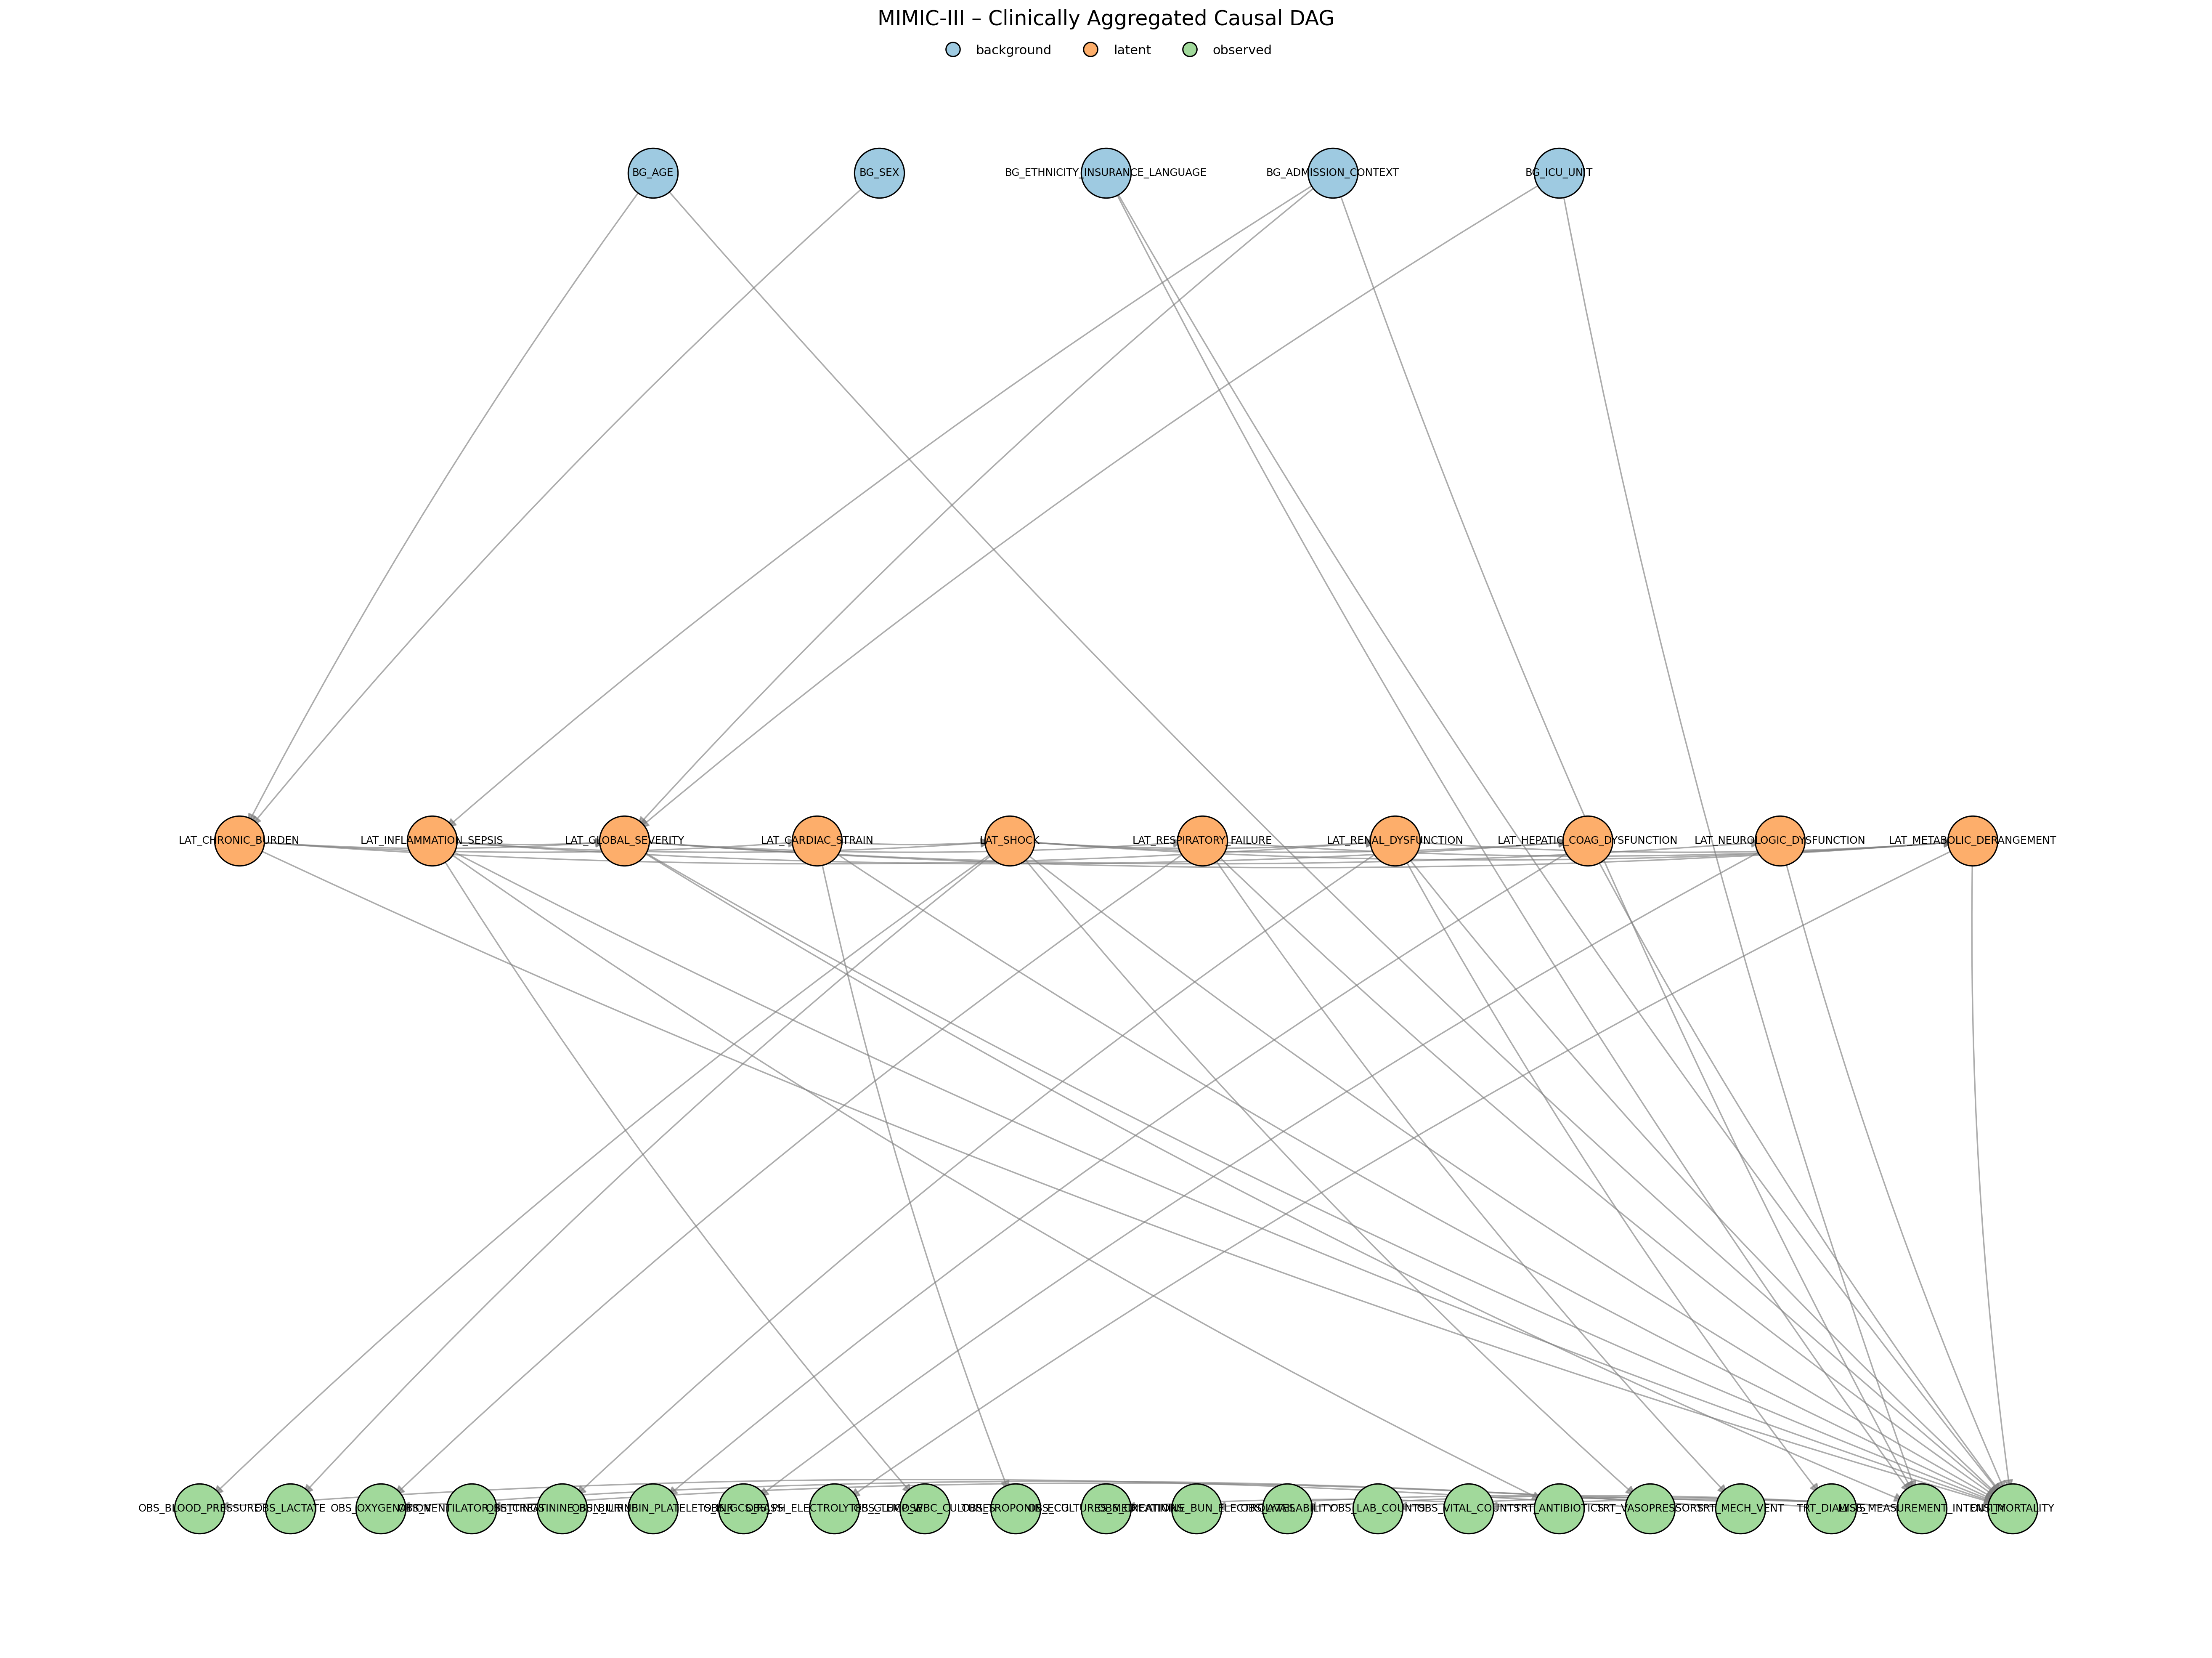
\includegraphics[
        width=\linewidth,
        height=0.82\textheight,
        keepaspectratio
    ]{figures/mimic_causal_dag.png}
    \caption{MIMIC-III dataset-specific causal DAG. Background and case-mix
    variables are shown in blue, latent clinical proxy variables in orange,
    and observed measurements, care-process variables, and mortality in green.
    The DAG was elicited as a high-level clinical representation and encoded
    for graph-based causal adjustment; it was not learned from the data or
    independently validated edge by edge.}
    \label{fig:mimic-causal-dag}
\end{figure}
\end{landscape}

\clearpage

\begin{landscape}
\begin{figure}[p]
    \centering
    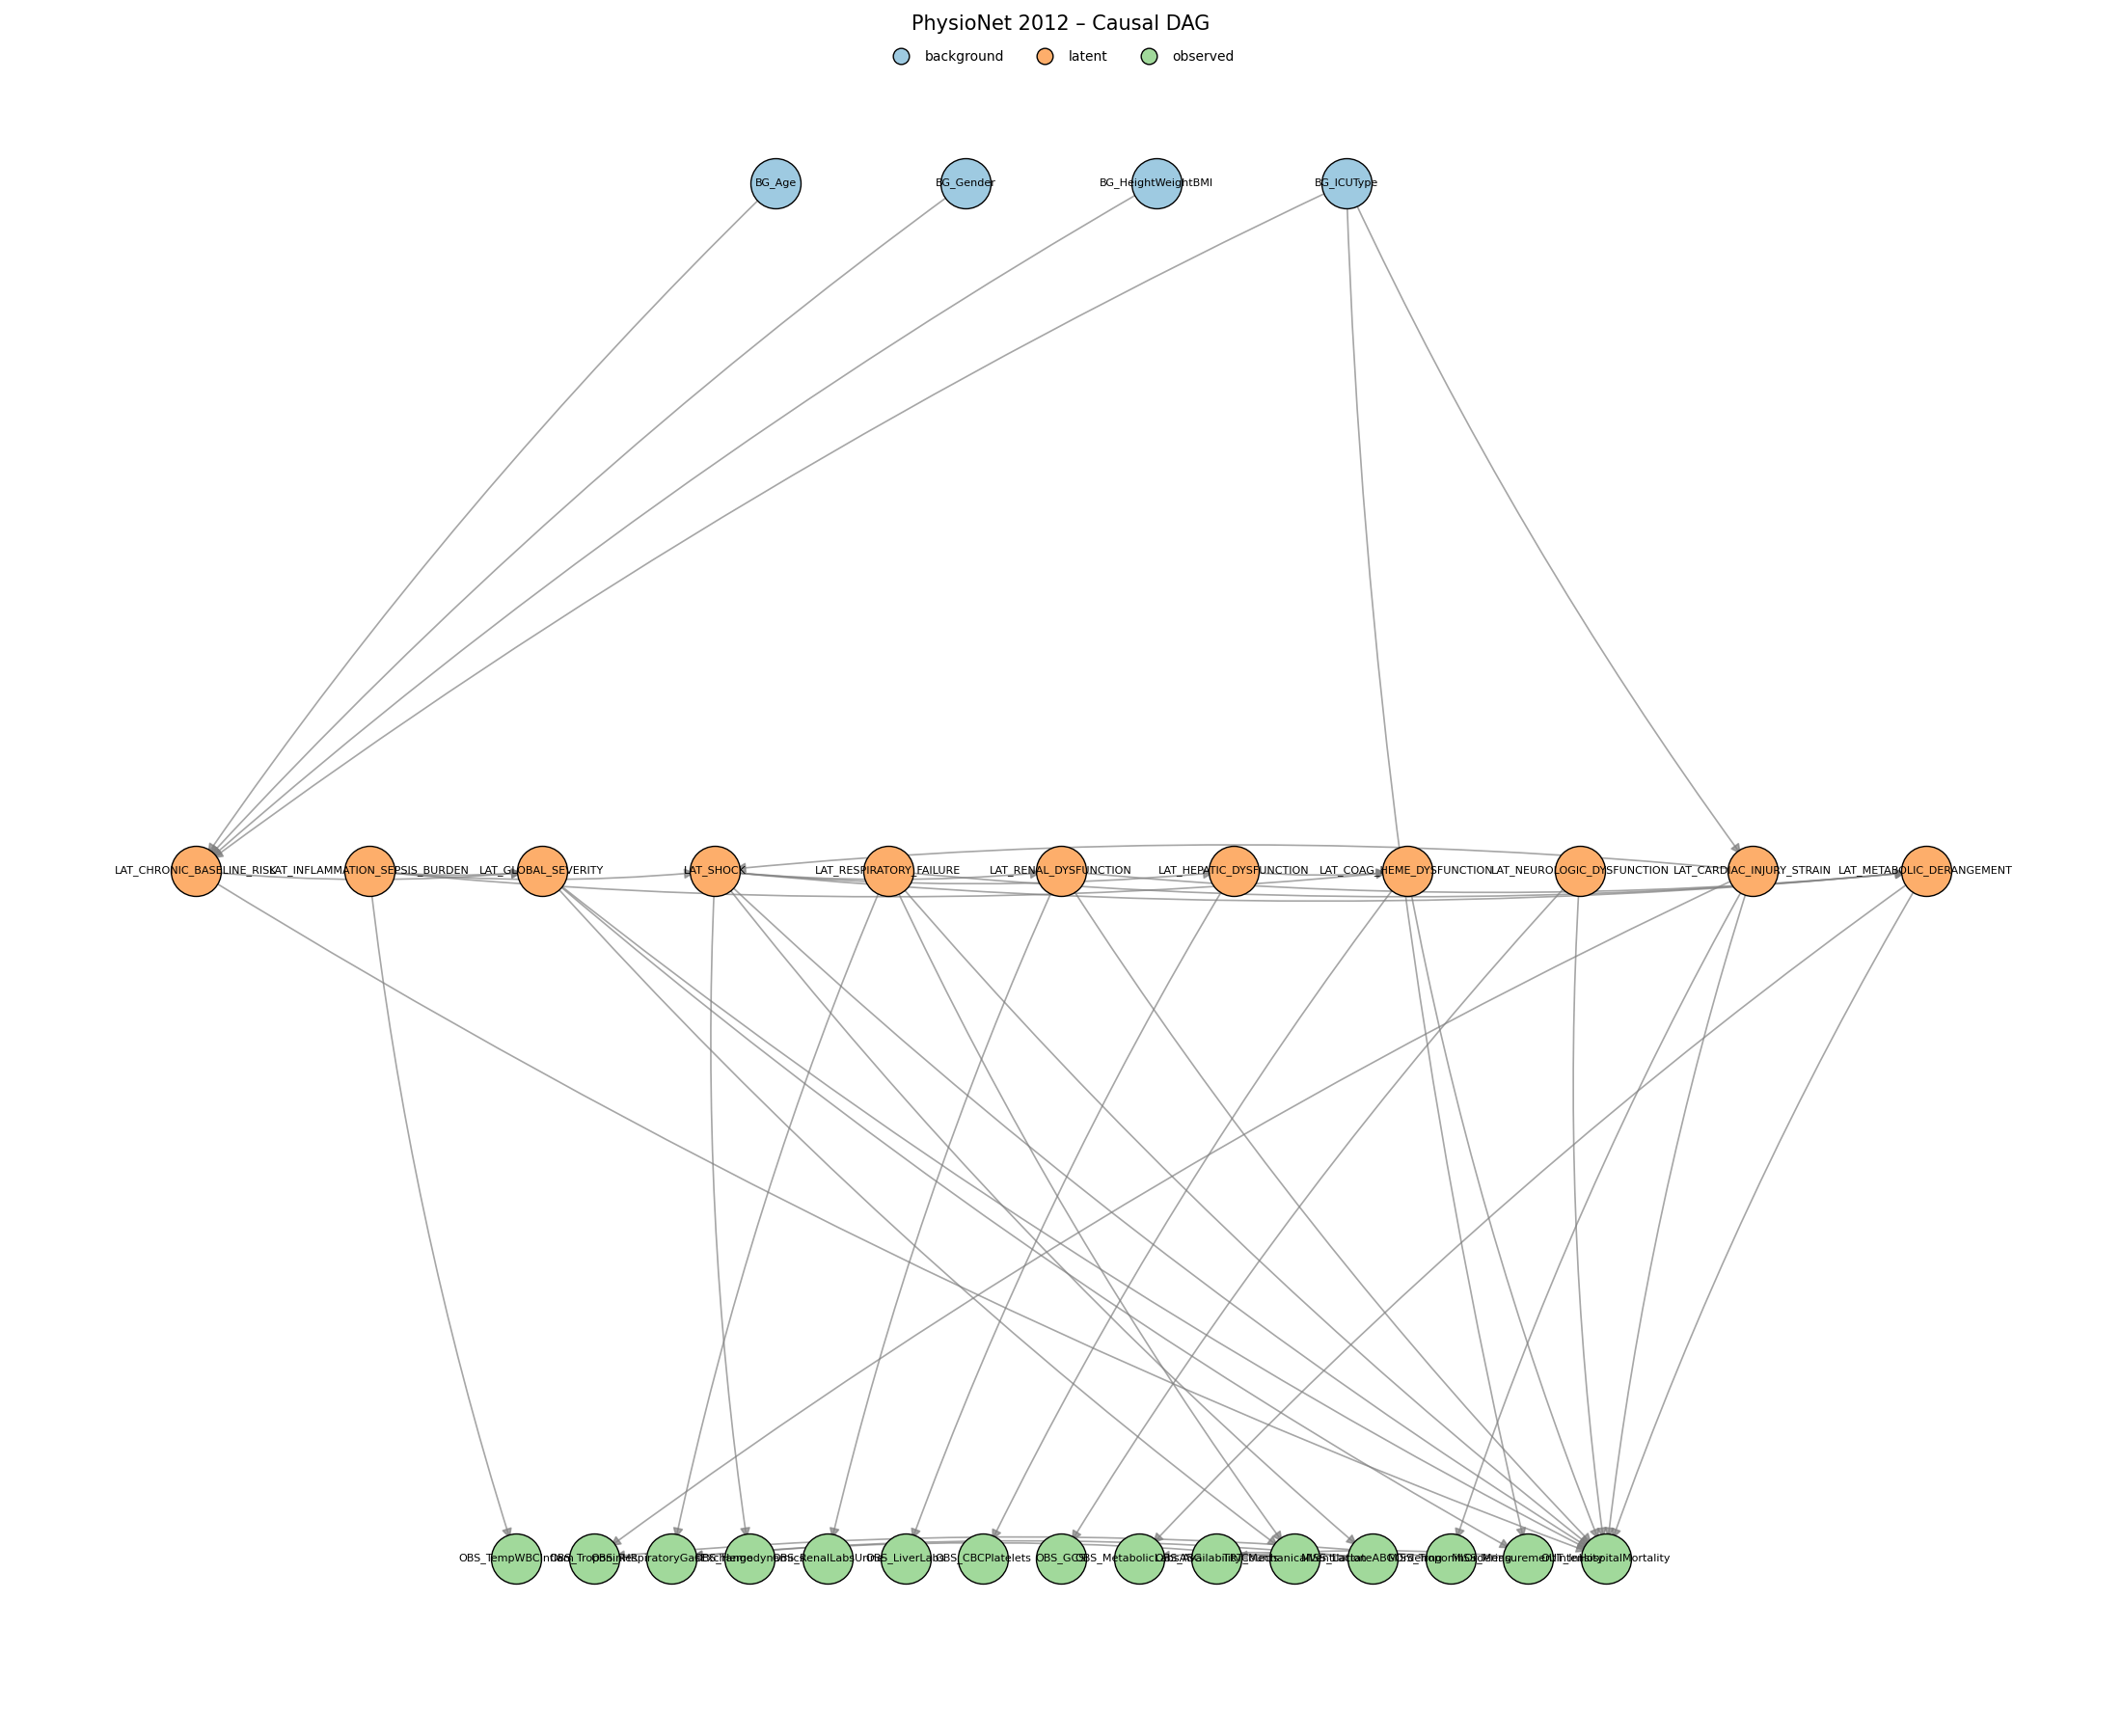
\includegraphics[
        width=\linewidth,
        height=0.82\textheight,
        keepaspectratio
    ]{figures/physionet_causal_dag.png}
    \caption{PhysioNet 2012 dataset-specific causal DAG. Background and
    case-mix variables are shown in blue, latent clinical proxy variables in
    orange, and observed measurements and mortality in green. The DAG was
    elicited as a high-level clinical representation and encoded for
    graph-based causal adjustment; it was not learned from the data or
    independently validated edge by edge.}
    \label{fig:physionet-causal-dag}
\end{figure}
\end{landscape}


\clearpage
\section{Computational Environment and Code Provenance}
\label{sec:supp-computation}

\subsection{Execution environment and hardware}

All experiments were executed through Python command-line programs orchestrated
by the CliniCause router, with Bash wrappers and Slurm used for server
submission. The submitted Slurm configuration requested one GPU, eight CPU
cores, 29\,GB of system memory, and a maximum wall time of 24 hours. The job ran
inside an Apptainer container with the project Conda environment mounted into
the container. The Slurm request did not require a particular GPU model;
depending on scheduler placement, the allocated accelerator was an NVIDIA RTX
6000 Ada Generation GPU or an NVIDIA A100 SXM4 GPU with 80\,GB of device memory.
The exact assigned accelerator and software-visible device state were recorded
in the job log using \texttt{nvidia-smi}.

The submitted one-GPU configuration set
\texttt{strats-max-concurrent=1}. Consequently, when both datasets were
requested, the router could maintain separate dataset processes and output
trees, but GPU-bound stages were protected by a process-safe lock and used the
single assigned accelerator serially.

The router additionally supports a parallel two-GPU configuration. In this
mode, it launches PhysioNet and MIMIC as separate child processes, assigns each
process a distinct GPU through \texttt{CUDA\_VISIBLE\_DEVICES}, and permits two
concurrent GPU stages. The corresponding expanded server allocation uses two
GPUs, 16 CPU cores, and 55\,GB of system memory. CPU-core and RAM allocations
are specified by Slurm; the router controls process creation, GPU assignment,
locking, logging, and separation of dataset-specific artifacts.

\subsection{Predictive-model implementations}

The STraTS, TCN, GRU, and GRU-D implementations originated from the public
STraTS repository:

\begin{center}
\url{https://github.com/sindhura97/STraTS}
\end{center}

The upstream code was adapted for the present study. The original supervised
task used a single binary mortality target. In our implementation, the target
columns are read from the dataset-specific latent-proxy CSV file, and the
prediction head produces a vector with one logit per proxy variable. The output
dimension is therefore the number of proxy targets rather than one mortality
logit. All four architectures share this modified prediction interface and are
trained using element-wise weighted binary cross-entropy with logits. The
per-target positive-class weights are estimated from the training partition,
and sigmoid probabilities are thresholded at 0.5 when binary proxy predictions
are exported.

The encoder implementations and their upstream provenance were retained, while
the multi-target proxy-prediction interface, split and artifact contracts,
checkpoint metadata, prediction export, and integration into CliniCause were
implemented for this study.

\subsection{Causal-analysis implementations}

The CliniCause orchestration layer and the project-specific causal pipeline were
implemented in Python for this study. This code covers dataset
adaptation, rule-based proxy generation, majority voting, dataset-specific DAG
construction, graph-based adjustment-set selection, matching diagnostics,
causal-effect estimation, result aggregation, permutation analyses, artifact
validation, and run-level provenance.

The matching implementation is project code contained in
\texttt{src/matching\_causal\_effect.py}. Matching is executed as a diagnostic
stage within each causal run and its outputs are stored under that run's
matching directory. It is not a separate estimator family, and no AIPW
estimator was used.

The two double-machine-learning estimators were imported from version 0.16.0 of
the EconML library, specifically:

\begin{itemize}
    \item \texttt{econml.dml.CausalForestDML};
    \item \texttt{econml.dml.LinearDML}.
\end{itemize}

The project configures these estimator classes and their nuisance models,
selects treatment-specific adjustment variables from the dataset DAG, fits the
estimators, and writes the treatment-level CATE outputs and diagnostics. The
underlying EconML estimator implementations were not reimplemented by us.

The CausalPFN estimator was imported as
\texttt{causalpfn.CATEEstimator} from CausalPFN version 0.1.4. Its upstream
implementation is available at:

\begin{center}
\url{https://github.com/vdblm/CausalPFN}
\end{center}

Our pipeline supplies the selected confounders and effect modifiers to the
pretrained CausalPFN estimator, invokes its fitting and CATE-estimation
interface, and integrates the returned estimates into the same run-specific
output and provenance structure used for the EconML estimators.

% Add the bibliography command used by the combined paper project here, e.g.:
\bibliographystyle{plain}
\bibliography{references}

% ============================================================
% Archived ChatGPT elicitation materials
% Insert this entire block after the bibliography and
% immediately before \end{document}.
% ============================================================

\clearpage
\appendix

\section*{Archived ChatGPT Elicitation Materials}
\addcontentsline{toc}{section}{Archived ChatGPT Elicitation Materials}

The following materials reproduce the ChatGPT elicitation artifacts used during
the representation-design stage. They are included separately from the authored
supplementary analyses and are preserved without substantive editing. The
general protocol was instantiated separately for MIMIC-III and PhysioNet 2012.
The resulting outputs document the proposed latent variables, operational proxy
rules, measurement model, missingness analysis, causal graph, and implementation
specifications. These archived outputs record the elicitation process; they do
not establish clinical validation or causal ground truth.

\subsection*{General Latent-Causal-Model Elicitation Prompt}
\addcontentsline{toc}{subsection}
  {General Latent-Causal-Model Elicitation Prompt}

The following reusable prompt was applied separately to the two datasets after
setting its dataset-name and official-description global variables.

\begingroup
\scriptsize
\VerbatimInput[
  breaklines=true,
  breakanywhere=true,
  breaksymbolleft={},
  tabsize=2
]{prompting/general-purpose-latent-causal-model-prompt.txt}
\endgroup


% ============================================================
% MIMIC-III archived ChatGPT output
% ============================================================

\clearpage
\thispagestyle{empty}

\begin{center}
    {\LARGE\bfseries MIMIC-III ChatGPT Elicitation Output}

    \vspace{1em}

    {\large Archived output corresponding to the general\\
    latent-causal-model elicitation protocol}
\end{center}

\vspace{2em}

% The first source-PDF page has a non-standard short page box,
% so import it separately as a graphic.
\noindent
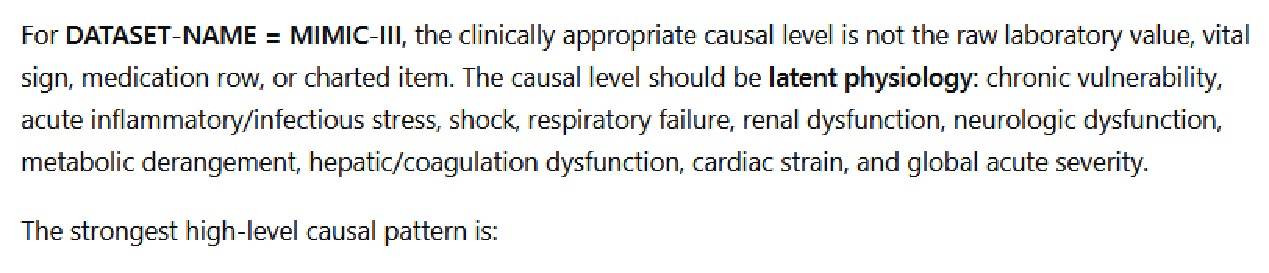
\includegraphics[
    page=1,
    width=\textwidth,
    keepaspectratio
]{prompting/clean-mimic-prompt-results.pdf}

\clearpage

% Pages 2 onward have normal portrait dimensions.
\includepdf[
    pages=2-,
    pagecommand={\thispagestyle{empty}}
]{prompting/clean-mimic-prompt-results.pdf}


% ============================================================
% PhysioNet 2012 archived ChatGPT output
% ============================================================

\clearpage
\thispagestyle{empty}

\begin{center}
    {\LARGE\bfseries PhysioNet 2012 ChatGPT Elicitation Output}

    \vspace{1em}

    {\large Archived output corresponding to the general\\
    latent-causal-model elicitation protocol}
\end{center}

\vspace{2em}

% The first source-PDF page also has a non-standard short page box.
\noindent
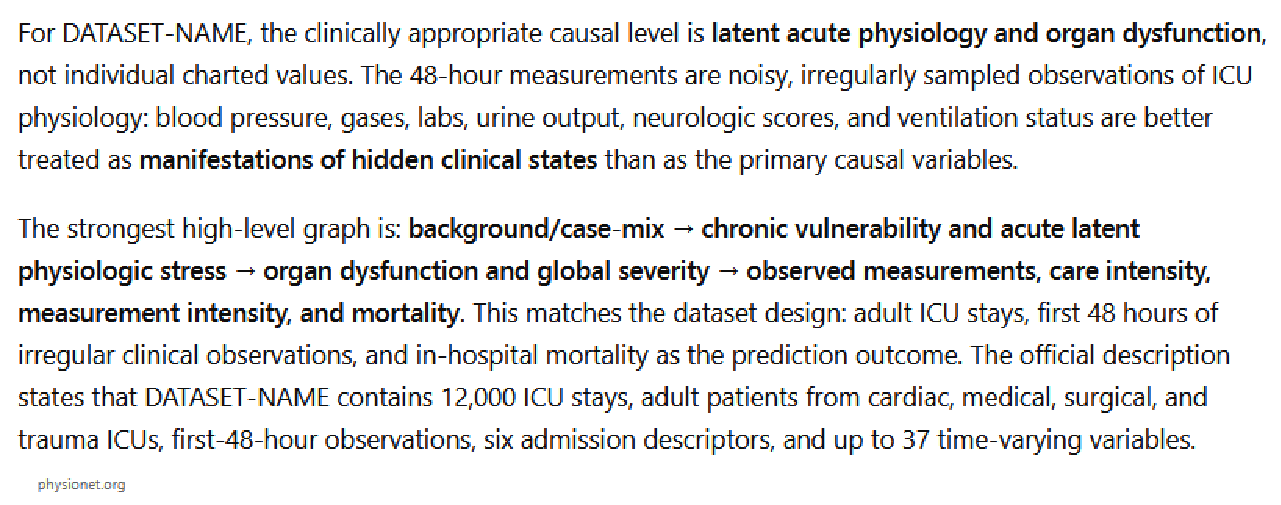
\includegraphics[
    page=1,
    width=\textwidth,
    keepaspectratio
]{prompting/clean-physionet-prompt-results.pdf}

\clearpage

% Pages 2 onward have normal portrait dimensions.
\includepdf[
    pages=2-,
    pagecommand={\thispagestyle{empty}}
]{prompting/clean-physionet-prompt-results.pdf}


\end{document}
